%!TEX root = ../thesis.tex
%*******************************************************************************
%****************************** Third Chapter **********************************
%*******************************************************************************
\chapter{Introduction}
The discovery of new pharmaceuticals traditionally follows the design-make-test paradigm, where molecules are repeatedly proposed, synthesized, and assayed. Drug candidates are designed based on some hypothesis relating chemical structure to drug activity, which gets updated in light of new activity results. This cycle repeats as the molecular search space narrows down until a candidate molecule satisfies the necessary activity/selectivity/toxicity criteria.

\begin{figure}[!h] % !h ~ force here, t ~ top, b ~ bottom, p ~ separate page
\centering
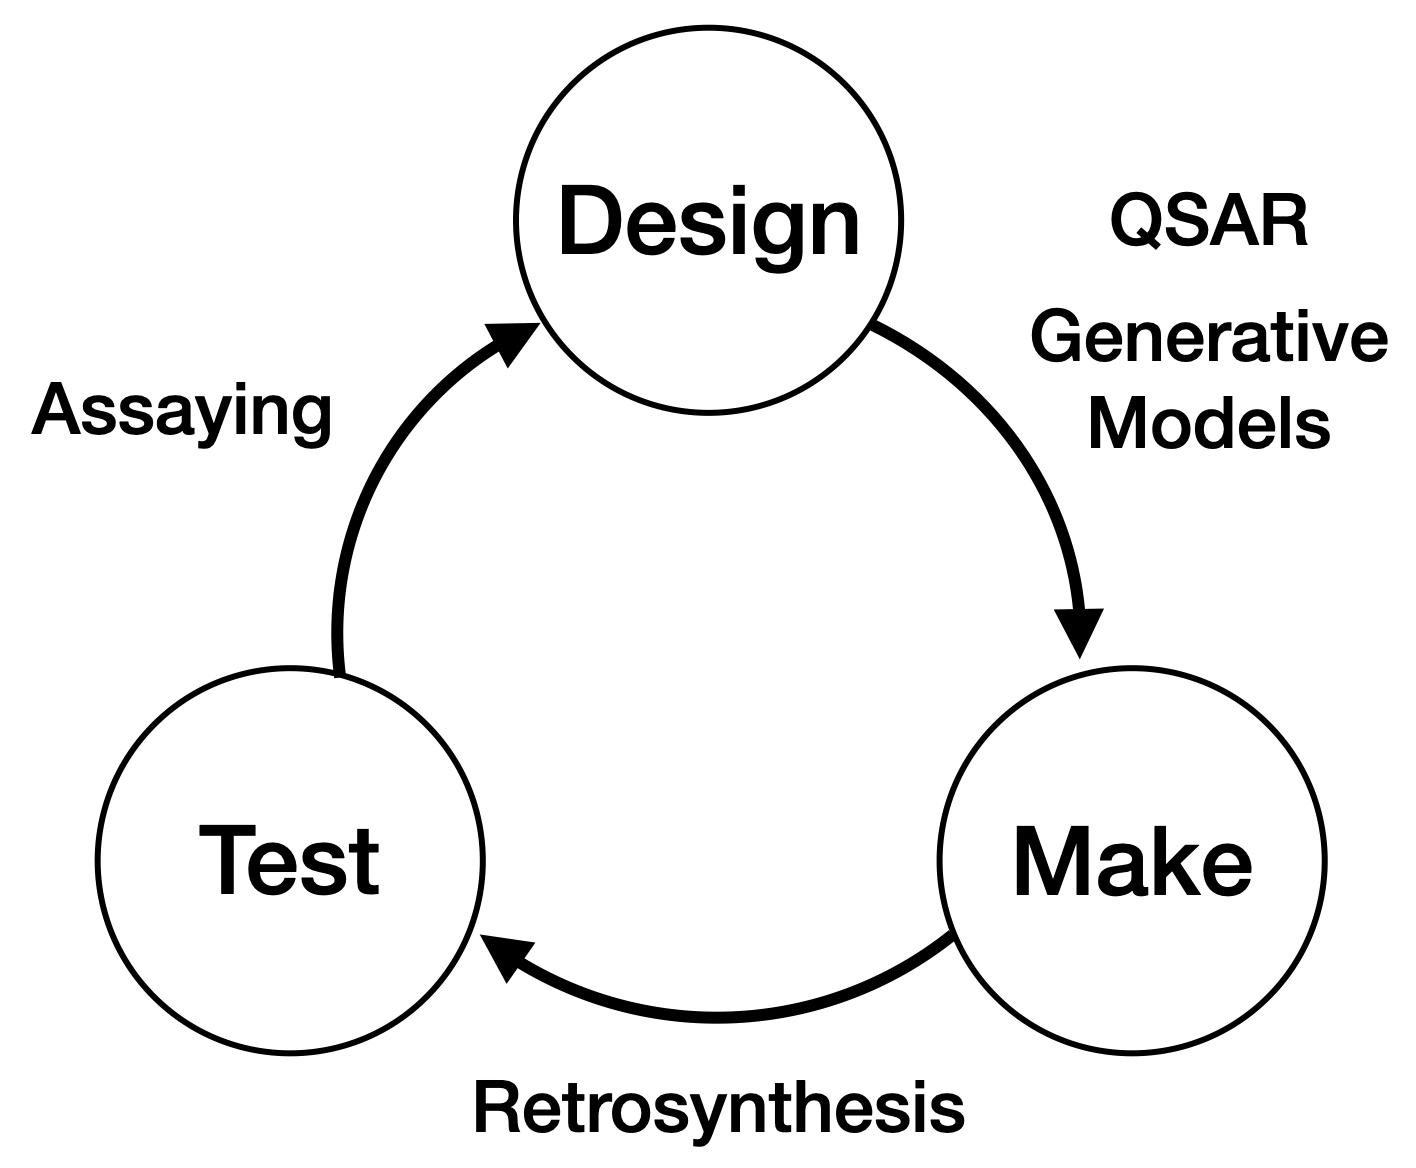
\includegraphics[width=0.5\textwidth]{Ch1/Figs/design-make-test.png}
\caption{\label{fig:cycle} An overview of the design-make-test cycle in drug discovery.}
\end{figure}

While computational methods have long been used in various stages of the cycle, there has been a recent surge in applying artificial intelligence to drug discovery following its success in various other fields, most notably computer vision and natural language processing. Since molecular assaying is largely an automated process the application focus has been on `design' and `make' \cite{Coley2019AutonomousProgress}, for example in modelling quantitative structure-activity relationships (QSAR), designing generative models for proposing drug candidates, and planning retrosynthesis routes (Fig~\ref{fig:cycle}). 

As the field of data-driven drug discovery matures beyond merely adapting the latest state-of-the-art machine learning (ML) methods, the present challenge is to tailor ML models specifically for the unique problems and situations faced in pharmaceutical chemistry. This report summarizes my efforts over the past year to play a part in this challenge with intuitions based on physical science. These consist of three separate tasks, one on `Make' and two on `Design':

\begin{itemize}
    \item \textbf{Interpreting learnt chemical principles from Molecular Transformer:} a state-of-the-art reaction prediction model (Molecular Transformer) was investigated with input and data attribution methods to discern whether the model had learnt chemically reasonable patterns of reactivity, or had simply succumbed to hidden bias in the datasets.
    \item \textbf{Exploiting molecular shape for property prediction:} a descriptor of atomic positions known as SOAP, which has seen widespread use in condensed matter physics due to its symmetry-invariance properties, was utilized in a Gaussian Processes model and shown to be competitive with other state-of-the-art models on predicting bioactivity. It was also demonstrated that ensembling models with diverse representations led to further predictive power.
    \item \textbf{Designing Sars-CoV-2 MPro inhibitors:} An initiative known as COVID Moonshot \cite{moonshot2020} was established to search for inhibitors of the Sars-CoV-2 main protease (MPro), crowd-sourcing drug candidate designs from the scientific community. In the early stages of the project, I utilised a genetic algorithm with SOAP descriptors for combining disparate fragment hits; in the most recent stage, I implemented a graph siamese network to learn how to rank the activity of assayed molecules, which was then used to suggest new candidates via computational screening of a constructed library.
\end{itemize}
The lessons learnt from these projects are used to inform possible avenues of future research, which are discussed in the final chapter of this report.